
\section{Muon System}

Muons at CMS~\cite{muon_tdr} are measured in the pseudorapidity range $\abs{\eta} < 2.4$, with detection planes made using three technologies: drift tubes, cathode strip chambers, and resistive plate chambers, as presented in Figure~\ref{cms_muon}. The single muon trigger efficiency exceeds 90\% over the full $\eta$ range, and the efficiency to reconstruct and identify muons is greater than 96\%. Matching muons to tracks measured in the silicon tracker results in a relative transverse momentum resolution, for muons with \pt up to 100\GeV, of 1\% in the barrel and 3\% in the endcaps. The \pt resolution in the barrel is better than 7\% for muons with \pt up to 1\TeV~\cite{Sirunyan:2018}. 

% cms muon
\begin{figure}[htbp]
    \centering
    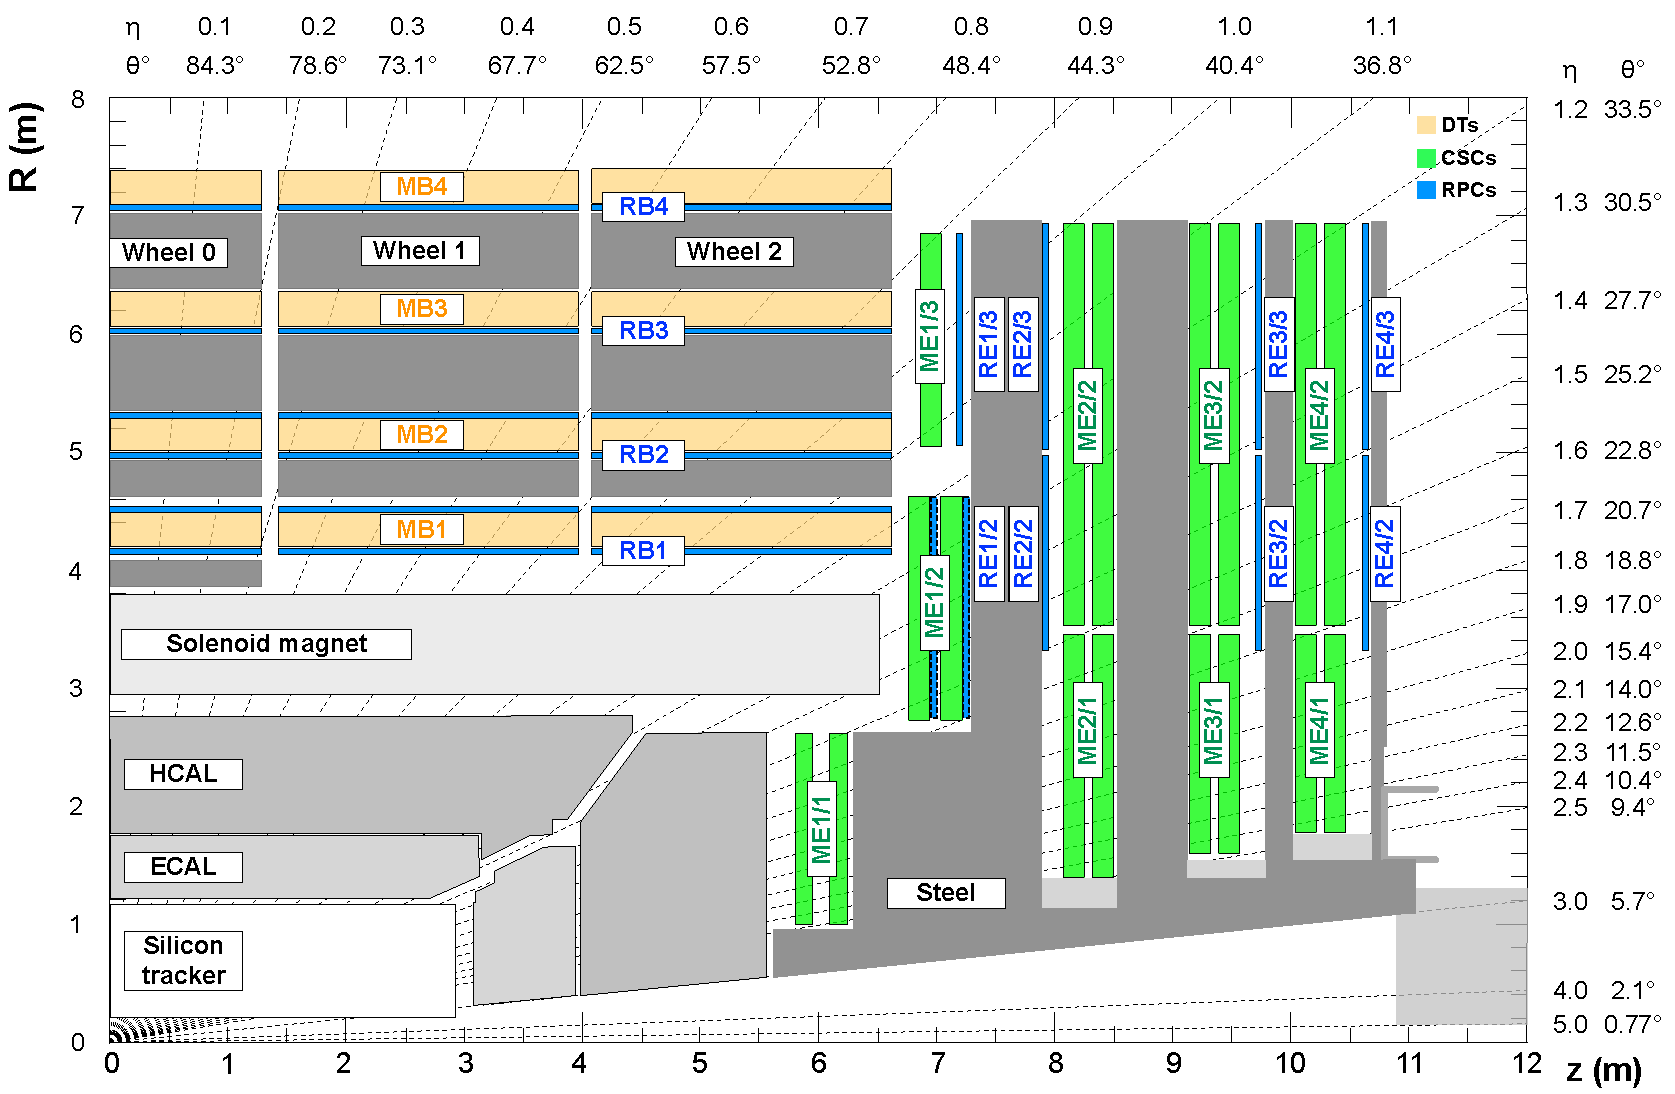
\includegraphics[width=\textwidth]{figures_and_tables/experimental_setup/cms_muon.pdf}
    \caption{Longitudinal section view of the ECAL and its components. Source:~\cite{Chatrchyan:2013sba}.}
    \label{cms_muon}
\end{figure}

The muon detection system has around 1 million channels. For Run3, the muon system is being expanded and upgraded, by the inclusion of new chamber with the Gas Electron Multiplier (GEM)~\cite{Sauli:2262884} technology.

\subsection{Drift Tubes}
\todo[inline]{FAZER!}

The Drift Tubes (DT)~\ref{Teyssier:2015xjj} are installed in the central region of CMS (Barrel), covering the region of $|\eta < 1.2|$. The barrel is divided in 5 wheels, along $z$, W+2, W+1, W0, W-1 and W-2. Each will is composed by four concentric stations along $r$, MB 1 to MB4, and each station is divided in 12 sectors along $\phi$, S01 to S12. In total, there are 205 DT chambers.

